\chapter{Evaluation}\label{evaluation}

This chapter focuses on the evaluation of the transfer pipeline. First, the individual steps of the pipeline are analyzed and evaluated to examine intermediate results and identify potential weaknesses, starting with an assessment of the scores assigned to the selected passages from the source datasets. Next, the different approaches for selecting candidate documents from the target document corpus are evaluated to determine the most effective approach.
\\\\
The evaluation of the candidate retrieval approaches can only be conducted by applying the transfer pipeline to a target dataset that already contains query relevance judgments. This is necessary because the goal of the candidate retrieval is to pre-select candidate documents from a target corpus that are likely to be relevant to a query. To measure this accurately, the target documents must be labeled with existing relevance judgments.
\\\\
The second part of the chapter focuses on the evaluation of the inferred relevance judgments through two transfer strategies. The first evaluation applies the transfer pipeline to a source dataset and uses the same dataset as the target. This self-transfer evaluation measures how well the pipeline reproduces known relevance judgments within the same dataset. The second evaluation assesses the final transfer to \texttt{ClueWeb22/b} as the target dataset. To facilitate this evaluation, a pooling process is conducted on the candidate documents selected by the best-performing candidate retrieval approach. This is followed by a manual relevance judgment of the pooled documents. The quality of the transferred relevance judgments to \texttt{ClueWeb22/b} is then evaluated based on these manual relevance judgments.
% ================
% Rank Correlation
% ================
\section{Rank Correlation}\label{rank-correlation}

\begin{table}[t]
  \centering
  \caption{Comparison of rank correlation metrics computed by Kendall's $\tau$ and Spearman's $\rho$. The table shows the rank correlation between the reference scores $[0.2,0.7,0.5]$ and three label sets: two with an expected correlation of $1$, and one with lower correlation. Default represents the actual rank correlation scores, while Greedy shows the scores obtained by greedily mapping the reference scores to the label set, representing the idealized rank correlation outcome.}
  \label{tab:rank-correlation}
  \begin{tabular}{ccccc}
      \toprule
      \textbf{Comparative Set} & \multicolumn{2}{c}{\textbf{Default}} & \multicolumn{2}{c}{\textbf{Greedy}} \\
      \cmidrule(lr){2-3} \cmidrule(lr){4-5}
                               & $\tau$ & $\rho$ & $\tau$ & $\rho$ \\
      \midrule
      
      $[0, 2, 1]$ & 1.00 & 0.99  & 1.00  & 1.00 \\
      $[0, 1, 1]$ & 0.82 & 0.92  & 1.00  & 1.00 \\
      $[0, 0, 1]$ & 0.00 & 0.11  & 0.50  & 0.50 \\
      \bottomrule
  \end{tabular}
\end{table}

Before starting with the evaluation of the transfer pipeline, I present the metrics used to evaluate the relevance judgments produced by the pipeline against the actual relevance judgments provided by the retrieval tasks. This clarification is important, as the evaluation results of the passage scores \mbox{(Section~\ref{passage-scoring})} and the final relevance judgments (Section~\ref{pairwise-preferences}) generated by the transfer pipeline are based on these metrics.
\\\\
\texttt{Inter-Annotator Agreement}~\citep{artstein:2017} is a statistical measure that quantifies the consistency among multiple annotators when labeling the same dataset. It provides insight into annotation quality by indicating the level of agreement or disagreement over all annotations. However, this measure requires all annotators to use the same categorical label set. In this thesis, retrieval tasks assign integer relevance labels ($\in \mathbb{N}$), while the inferred relevance labels are continuous scores ($\in \mathbb{R}^{+}$). Due to this mismatch, the \mbox{\texttt{Inter-Annotator Agreement}} is unsuitable for evaluation.
\\\\
Instead, \texttt{Rank Correlation} is used to compare actual relevance labels with the inferred relevance scores. \texttt{Rank Correlation} evaluates how well two rankings align. Here, the retrieval task's relevance judgments serve as the ground truth, against which the transfer pipeline's inferred judgments are compared. The correlation metrics used are \texttt{Kendall's $\tau$} and \texttt{Spearman's $\rho$}. Both metrics compute the rank correlation between linear orders~\citep{monjardet:1998}, making them well-suited for the retrieval task labels and inferred scores. A high rank correlation indicates that the generated judgments preserve the ranking order of the original relevance labels, what is the goal.
\\\\
Table~\ref{tab:rank-correlation} illustrates how these metrics assess sample relevance judgments. It presents agreement between example reference scores $[0.2, 0.7, 0.5]$ and three label sets: the first two yielding an expected correlation of $1$, while the third exhibits a lower correlation. The \texttt{Default} column contains correlation scores computed by standard \texttt{Kendall's $\tau$} and \texttt{Spearman's $\rho$} algorithms. Unlike the default algorithms, the goal in this thesis is to maximize alignment between inferred relevance scores and ground truth labels. For instance, the relevance scores $[0.2, 0.7, 0.5]$ should ideally correspond to the label set $[0, 1, 1]$ (second row of Table~\ref{tab:rank-correlation}). This alignment can be achieved by mapping scores less than or equal to $0.2$ to label $0$ and scores greater than $0.2$ to label $1$. Therefore, the intended rank correlation for this example should be $1$.
\\\\
To accomplish this, a modified version called \texttt{Greedy} was tested alongside the default algorithms. This variant greedily maps the relevance scores to the label set, producing the highest possible correlation. The example demonstrates that standard correlation metrics are sensitive to the rank order of relevance judgments, whereas the \texttt{Greedy} version eliminates this sensitivity, achieving the maximum correlation scores.

% Before starting with the evaluation of the transfer pipeline, I present the metrics used to evaluate the relevance judgments produced by the pipeline against the actual relevance judgments provided by the retrieval tasks. This clarification is important, as the evaluation results of the passage scores \mbox{(Section~\ref{passage-scoring})} and the final relevance judgments (Section~\ref{pairwise-preferences}) generated by the transfer pipeline are based on these metrics.
% \\\\
% The \texttt{Inter-Annotator Agreement}~\citep{artstein:2017} is a statistical measure that quantifies the consistency between annotations provided by multiple annotators. It indicates the level of agreement or disagreement among annotators when labeling the same dataset, thereby offering insight into the quality of the annotations. In this thesis, the ground truth annotation is represented by the relevance judgments provided by the retrieval tasks. These judgments are compared to the inferred relevance judgments generated by the transfer pipeline. A high \texttt{Inter-Annotator Aggreement} score indicates a strong agreement between the actual relevance labels and the inferred relevance labels.
% \\\\
% Various methods exist for calculating \texttt{Inter-Annotator Aggreement}, each with its strengths and weaknesses. In this thesis, the retrieval tasks provide judgments as integer labels, i.e., $\in \mathbb{N}$, while the inferred relevance labels are represented as actual relevance scores, i.e., $\in \mathbb{R}^{+}$. Consequently, not every correlation method is suitable for computing the aggreement between the relevances. Therefore, the correlation metrics used to evaluate the level of agreement are \texttt{Kendall's $\tau$} and \texttt{Spearman's $\rho$}. Both metrics compute the rank correlation between linear orders~\citep{monjardet:1998}, making them well-suited to the nature of the retrieval tasks labels and inferred relevance scores in this thesis.
% \\\\
% Table~\ref{tab:rank-correlation} presents an example of how the correlation metrics are calculated based on some sample labels of the relevance judgments. The table shows the agreement between example reference scores $[0.2, 0.7, 0.5]$ and three label sets: the first two with an expected correlation of $1$, and the last one with lower correlation. The \texttt{Default} column represents the actual rank correlation scores computed by the standard algorithms of \texttt{Kendall's $\tau$} and \texttt{Spearman's $\rho$}.
% \\\\\\\\\\\\\\
% In contrast to the default algorithms, the desired rank correlation for this thesis, is characterized by the ability to map the inferred relevance scores to the actual relevance labels from the retrieval task in the best possible way. For example, the relevance scores $[0.2, 0.7, 0.5]$ should be perfectly mapped to the label set $[0, 1, 1]$ in the second row of Table~\ref{tab:rank-correlation}. This could be achieved by assuming that all relevance scores smaller equal $0.2$ correspond to label $0$ and all scores greater $0.2$ correspond to label $1$. Therefore, the intended rank correlation for this example should be $1$, in this thesis. To achieve this, a modified variant called \texttt{Greedy} was tested alongside the default versions. This variant greedily maps the reference scores to the label set, representing the idealized rank correlation outcome. This example demonstrates that the default correlation metrics are sensitive to the rank order of the relevance judgments, whereas the \texttt{Greedy} variant avoids this sensitivity, achieving the maximum possible correlation scores.


% ==================
% Document Selection
% ==================
\section{Document Selection}\label{eval-document-selection}

The first step in the transfer pipeline was selecting and segmenting a subset of documents for each query in a retrieval task from the source dataset. These selected documents play a crucial role in two subsequent steps, identifying candidate documents from the target corpus and performing pairwise preference comparisons using \texttt{DouPrompt}. Since only a subset of documents is required per query, two selection criteria were applied. First, only documents with at least one relevance judgment in the \texttt{qrel store} were considered, as documents without judgments do not provide transferable information. Second, a maximum of 50 relevance judgments per relevance label per query, referred to as a query-label combination, was selected to manage computational complexity.
\\\\\\\\\\\\\\\\\\
Table~\ref{tab:document-selection} presents the results of this selection process. On average, close to 50 documents per query-label combination were selected, ensuring a balanced representation of relevant and non-relevant judgments. Ideally, each query should have approximately 50 non-relevant documents and at least 50 relevant ones. All \texttt{TREC} retrieval tasks performed well, providing the maximum number of non-relevant documents per query. Additionally, \texttt{TREC-19 DL} and \texttt{TREC-20 DL} exceeded the \mbox{threshold} of 50 relevant documents per query, ensuring a diverse pool for candidate retrieval and pairwise comparisons. Similarly, \texttt{TREC-7} and \texttt{TREC-8} achieved strong results, with an average of over 40 relevant documents. \texttt{Robust04} contains a substantial number of relevance judgments for its 250 queries, though most are non-relevant. Nonetheless, it maintains a solid average of over 36 relevant documents per query for further processing. The only outlier is \texttt{Touché 20}, which averages just 28 non-relevant and 19 relevant judgments per query.
\\\\
The lower numbers for \texttt{Touché 20} limit the effectiveness of the nearest neighbor candidate retrieval approach and the pairwise preference comparisons. This is due to the low amount of relevance judgments available in the retrieval task. However, given the relatively small size of \texttt{Args.me} (0.4 million documents), the transfer pipeline's results may remain valuable.
\\\\
This intermediate evaluation confirms that the selection process successfully provides an adequate number of documents for subsequent steps in the pipeline. While \texttt{Touché 20} remains useful, its results should be interpreted cautiously due to the lower document count per query.

% The first step in the transfer pipeline was the selection and segmentation of a subset of documents for each query of a retrieval task from the source dataset. The selected documents play a crucial role in two subsequent steps of the pipeline. First, the selection of candidate documents from the target corpus and second the pairwise preference comparison using \texttt{DouPrompt}. Since only a subset of documents is necessary for each query, two selection conditions were applied. First, only documents with at least one relevance judgment in the \texttt{qrel store} of a retrieval task were considered for selection, as documents without relevance judgments do not have information to transfer. Second, a maximum of 50 relevance judgments per relevance label for each query (referred to as a query-label combination) was selected to limit the number of processed documents.
% \\\\
% The results of the selection process under these conditions are presented in Table~\ref{tab:document-selection}. An average close to 50 documents per query-label combination is possible. In order to have a wide selection of relevant and non-relevant judgments, an average close to 50 documents of non relevant judgments, i.e., documents, and close to or over (if the retrieval tasks has multiple levels of relevant) 50 relevant judgments, i.e., documents per query is aimed for. All \texttt{TREC} retrieval tasks achieve very good results, with providing the maximum of possible non relevant documents for each query. Also, \texttt{TREC-19 DL} and \texttt{TREC-20 DL} also reach in sum total over 50 relevant documents per query, thereby providing a wide range of documents for the candidate retreival step and also possiblilites for the pairwise comparisons at the end. \texttt{TREC-7} and \texttt{TREC-8} are also well performing with an average of over 40 documents per query-label combination. \texttt{Robust04} has a very large amount of relevance judgments for its 250 queries, but most of them are non-relevant judgments. Nevertheless, it achieves a good average of over 36 relevant documents to further process. The only outliner is \texttt{Touché 20} which just receives an average of 28 non relevant and 19 relevant judgments.
% \\\\
% The low numbers of \texttt{Touché 20} limit the possibilities for the nearest neighbor candidate retrieval approach and pairwise preferences combination. The low averages are due to the limited number of relevance judgments provided by the retrieval tasks, see Tabel~\ref{tab:datasets}. But due to the small size of \texttt{Args.me} with just $0.4$ million documents, the outcome of the transfer pipeline is still valuable.
% \\\\
% This intermediate evaluation step shows that the selection process is overall successful in providing a sufficient number of documents for the subsequent steps of the transfer pipeline. The outliner \texttt{Touché 20} is still valuable for the evaluation, but the results should be interpreted with caution due to the low number of documents per query.

\begin{table}[t]
  \centering
  \caption{The table presents the results of the candidate selection process, showing for each label of a retrieval task the number of documents per query for each source dataset. A maximum of 50 documents per query-label combination is possible.}
  \label{tab:document-selection}
  \resizebox{\textwidth}{!}{%
  \begin{tabular}{lcccccc}
      \toprule
      \textbf{Docs./Query} & \textbf{Touché 20} & \textbf{Robust04} & \textbf{TREC-7} & \textbf{TREC-8} & \textbf{TREC-19 DL} & \textbf{TREC-20 DL}  \\

      \midrule

      Label 0        & $27.9$ & $50.0$ & $50.0$ & $50.0$ & $ 49.6$ & $ 50.0$ \\
      Label 1        & $ 6.0$ & $32.8$ & $40.2$ & $40.5$ & $ 31.1$ & $ 28.5$ \\
      Label 2        & $13.0$ & $ 3.8$ &    -   &    -   & $ 23.8$ & $ 16.0$ \\
      Label 3        &    -   &    -   &    -   &    -   & $ 11.7$ & $ 10.3$ \\
      \midrule
      \textbf{Total} & $46.9$ & $86.6$ & $90.2$ & $90.5$ & $116.2$ & $104.8$ \\

      \bottomrule
  \end{tabular}}
\end{table}

%\\\\
% The segmentation of the selected documents was performed using the \texttt{trec-cast-tools} GitHub repository\footnote{\url{https://github.com/grill-lab/trec-cast-tools}}, which splits documents into passages of up to 250 words in length. This segmentation process is independent of the transfer pipeline and is therefore not evaluated in this thesis.
\pagebreak

% ===============
% Passage Scoring
% ===============
\section{Passage Scoring}\label{eval-passage-scoring}

\begin{table}[t]
    \centering
    \caption{Average rank correlations between the assigned passage scores and the original relevance judgments across all queries of a retrieval task, reported using Kendall's $\tau$ and Spearman's $\rho$.}
    \label{tab:passage-scoring}
    \resizebox{\textwidth}{!}{%
    \renewcommand{\arraystretch}{1.2}
    \begin{tabular}{clcccccccccccccc}
        \toprule
        \multicolumn{2}{c}{\textbf{Retrieval Model}} & \multicolumn{2}{c}{\textbf{Touché 20}} & \multicolumn{2}{c}{\textbf{Robust04}} & \multicolumn{2}{c}{\textbf{TREC-7}} & \multicolumn{2}{c}{\textbf{TREC-8}} & \multicolumn{2}{c}{\textbf{TREC-19 DL}} & \multicolumn{2}{c}{\textbf{TREC-20 DL}} & \multicolumn{2}{c}{\textbf{Avg.}} \\
        \cmidrule(lr){3-4} \cmidrule(lr){5-6} \cmidrule(lr){7-8} \cmidrule(lr){9-10} \cmidrule(lr){11-12} \cmidrule(lr){13-14} \cmidrule(lr){15-16}
                                                   & & $\tau$ & $\rho$ & $\tau$ & $\rho$ & $\tau$ & $\rho$ & $\tau$ & $\rho$ & $\tau$ & $\rho$ & $\tau$ & $\rho$ & $\tau$ & $\rho$ \\
        \midrule
        \multirow{10}{*}{\rotatebox{90}{\texttt{ndcg@10}}}
            & BM25         & 0.802 & 0.871 & 0.823 & 0.907 & 0.801 & 0.896 & 0.813 & 0.906 & 0.725 & 0.831 & 0.755 & 0.846 & 0.787 & 0.876 \\
            & DFR\_BM25    & 0.804 & 0.874 & 0.822 & 0.907 & 0.800 & 0.896 & 0.813 & 0.906 & 0.727 & 0.833 & 0.755 & 0.846 & 0.787 & 0.877 \\
            & DFIZ         & 0.778 & 0.852 & 0.820 & 0.906 & 0.796 & 0.896 & 0.800 & 0.898 & 0.730 & 0.836 & 0.753 & 0.845 & 0.780 & 0.872 \\
            & DLH          & 0.839 & 0.901 & 0.831 & 0.913 & 0.810 & 0.903 & 0.825 & 0.915 & 0.735 & 0.839 & 0.754 & 0.845 & 0.799 & 0.886 \\
            & DPH          & 0.783 & 0.856 & 0.820 & 0.905 & 0.799 & 0.895 & 0.809 & 0.903 & 0.725 & 0.831 & 0.753 & 0.844 & 0.782 & 0.872 \\
            & DirichletLM  & 0.679 & 0.752 & 0.816 & 0.902 & 0.798 & 0.896 & 0.802 & 0.898 & 0.721 & 0.825 & 0.751 & 0.841 & 0.761 & 0.852 \\
            & Hiemstra\_LM & 0.855 & 0.914 & 0.829 & 0.912 & 0.807 & 0.902 & 0.819 & 0.910 & 0.729 & 0.834 & 0.759 & 0.849 & \textbf{0.800} & \textbf{0.887} \\
            & LGD          & 0.801 & 0.874 & 0.819 & 0.905 & 0.799 & 0.897 & 0.802 & 0.899 & 0.730 & 0.835 & 0.757 & 0.848 & 0.785 & 0.876 \\
            & PL2          & 0.805 & 0.873 & 0.826 & 0.909 & 0.804 & 0.898 & 0.822 & 0.913 & 0.727 & 0.833 & 0.757 & 0.848 & 0.790 & 0.879 \\
            & TF\_IDF      & 0.807 & 0.876 & 0.823 & 0.907 & 0.801 & 0.896 & 0.814 & 0.907 & 0.726 & 0.832 & 0.755 & 0.847 & 0.788 & 0.877 \\
        \midrule
        \multirow{10}{*}{\rotatebox{90}{\texttt{precision@10}}}
            & BM25         & 0.765 & 0.828 & 0.807 & 0.881 & 0.792 & 0.872 & 0.807 & 0.885 & 0.657 & 0.756 & 0.697 & 0.785 & 0.754 & 0.835 \\
            & DFR\_BM25    & 0.768 & 0.833 & 0.806 & 0.880 & 0.791 & 0.870 & 0.807 & 0.884 & 0.658 & 0.757 & 0.696 & 0.785 & 0.754 & 0.835 \\
            & DFIZ         & 0.729 & 0.798 & 0.801 & 0.874 & 0.785 & 0.863 & 0.791 & 0.869 & 0.661 & 0.760 & 0.695 & 0.784 & 0.744 & 0.824 \\
            & DLH          & 0.802 & 0.862 & 0.817 & 0.889 & 0.803 & 0.881 & 0.823 & 0.899 & 0.666 & 0.764 & 0.697 & 0.785 & \textbf{0.768} & \textbf{0.847} \\
            & DPH          & 0.745 & 0.814 & 0.803 & 0.876 & 0.787 & 0.867 & 0.801 & 0.878 & 0.659 & 0.758 & 0.697 & 0.785 & 0.749 & 0.830 \\
            & DirichletLM  & 0.640 & 0.705 & 0.796 & 0.868 & 0.785 & 0.863 & 0.791 & 0.867 & 0.652 & 0.750 & 0.691 & 0.778 & 0.726 & 0.805 \\
            & Hiemstra\_LM & 0.819 & 0.880 & 0.813 & 0.886 & 0.799 & 0.878 & 0.815 & 0.892 & 0.658 & 0.757 & 0.699 & 0.786 & 0.767 & 0.846 \\
            & LGD          & 0.765 & 0.833 & 0.800 & 0.873 & 0.787 & 0.866 & 0.792 & 0.870 & 0.659 & 0.758 & 0.697 & 0.785 & 0.750 & 0.831 \\
            & PL2          & 0.766 & 0.829 & 0.811 & 0.885 & 0.796 & 0.876 & 0.819 & 0.896 & 0.656 & 0.755 & 0.698 & 0.786 & 0.758 & 0.838 \\
            & TF\_IDF      & 0.769 & 0.832 & 0.808 & 0.881 & 0.793 & 0.872 & 0.808 & 0.885 & 0.657 & 0.756 & 0.697 & 0.785 & 0.755 & 0.835 \\

        \bottomrule
    \end{tabular}}
    \renewcommand{\arraystretch}{1.0}
\end{table}

The next step in the transfer pipeline was to assign relevance scores to the passages of the selected documents from the previous step. This was done to identify the most relevant passages of a document with respect to the actual query associated with a document's relevance judgment. To achieve this, each passage was treated as an independent query and used to retrieve a document ranking from its original source corpus. Based on the retrieved document rankings, \texttt{precision@10} and \texttt{nDCG@10} were computed and assigned as passage scores. Since this study does not aim to optimize or analyze specific retriever systems but rather utilizes them for passage scoring, a diverse selection of models was tested, as listed in Table~\ref{tab:passage-scoring}.
\\\\
To evaluate the quality of the assigned passage scores and determine which retrieval model and metric combination were most effective in determining the relevance of passages, the rank correlation between the original relevance judgments and the newly assigned scores was computed using Kendall's $\tau$ and Spearman's $\rho$. For each retriever-metric combination, an overall document score was aggregated from its passage scores by selecting the maximum passage score. The rank correlation was then computed for all judged \mbox{documents} of each query individually, rather than across all relevance judgments of a retrieval task simultaneously, and then averaged. Macro-averaging across all queries is intended to reduce the effect of potential outliers for individual queries.
% \\\\
% To ensure a robust evaluation of the assigned passage scores, a 5-fold cross-validation was applied across the metrics, aggregation methods, and transformation methods for each combination of retrieval model and retrieval task. First, queries within each retrieval task were divided into five equal subsets (folds). For each fold, one subset was designated as the validation set, while the remaining four subsets formed the training set. In each iteration of the cross-validation, the metric, aggregation method, and transformation method that achieved the highest average correlation score on the training set (four-fifths of the queries) were selected. This selection process involved computing the average correlation score across all queries in the training set for each combination. The chosen combination was then evaluated on the test set (the remaining fifth of the queries) to obtain a final correlation score for that iteration. This process was repeated for all five folds, ensuring that each query subset served as the validation set exactly once. The final cross-validation score for each retrieval model and retrieval task was computed as the average correlation score across all five folds, thereby reducing the impact of overfitting and providing a more reliable estimate of passage scoring performance.
\\\\
The results in Table~\ref{tab:passage-scoring} show that all retrieval models achieved a very high rank correlation across all tested information retrieval tasks. While \texttt{Hiemstra\_LM} was the best-performing model, all models demonstrated strong performance based on the average $\tau$ and $\rho$ values. Therefore, the choice of retrieval model is not a critical factor for subsequent steps in the transfer pipeline, as all models produced passage scores with high rank correlation to the actual relevance labels from the retrieval tasks. This finding also applies to the \texttt{greedy} variant of both rank correlation methods, as shown in Table~\ref{tab:app:passage-scoring}. Although the greedy variant resulted in slightly higher rank correlation scores than the standard version, the overall behavior remained consistent.
\\\\
However, the choice of metric had a significant impact. \texttt{precision@10} consistently resulted in lower rank correlation compared to \texttt{nDCG@10}. This outcome was expected, as \texttt{precision@10} lacks the granularity needed to effectively differentiate between individual passages. Consequently, \texttt{nDCG@10} is the better metric for passage scoring. In the following steps of the transfer pipeline, the passage scores assigned by \texttt{nDCG@10} alongside the retrieval model that achieved the highest rank correlation for each retrieval task is therefore used.
\pagebreak


% ===================
% Candidate Selection
% ===================
\section{Candidate Selection}\label{eval-candidate-selection}

\begin{table}[t]
    \centering
    \footnotesize
    \caption{Overview of recall (Rec.) and the average number of candidate documents per query (Docs.) for all three candidate retrieval approaches, tested with document selection restricted to one passage per document (opd.) and without restriction (def.). The \texttt{Nearest Neighbor} and the \texttt{Union} approaches were also evaluated with varying $k$, determining the number of passages used for candidate retrieval.}
    \label{tab:candidate-selection}
    \resizebox{\textwidth}{!}{%
    \renewcommand{\arraystretch}{1.2}
    \begin{tabular}{ccrcrcrcrcrcrcr}
        \toprule

        \multicolumn{3}{c}{\textbf{Approach}} & \multicolumn{2}{c}{\textbf{Touché 20}} & \multicolumn{2}{c}{\textbf{Robust04}} & \multicolumn{2}{c}{\textbf{TREC-7}} & \multicolumn{2}{c}{\textbf{TREC-8}} & \multicolumn{2}{c}{\textbf{TREC-19 DL}} & \multicolumn{2}{c}{\textbf{TREC-20 DL}} \\

        \cmidrule(lr){4-5} \cmidrule(lr){6-7} \cmidrule(lr){8-9} \cmidrule(lr){10-11} \cmidrule(lr){12-13} \cmidrule(lr){14-15}
                                          & & $k$ & Rec. & Docs. & Rec. & Docs. & Rec. & Docs. & Rec. & Docs. & Rec. & Docs. & Rec. & Docs. \\
        \midrule
        \multirow{2}{*}{\rotatebox{90}{\textbf{Naive}}} & \multirow{2}{*}{-} & \multirow{2}{*}{-} & \multirow{2}{*}{$0.912$} & \multirow{2}{*}{$1\,556$} & \multirow{2}{*}{$0.777$} & \multirow{2}{*}{$1\,572$} & \multirow{2}{*}{$0.657$} & \multirow{2}{*}{$1\,600$} & \multirow{2}{*}{$0.713$} & \multirow{2}{*}{$1\,566$} & \multirow{2}{*}{$0.736$} & \multirow{2}{*}{$976$} & \multirow{2}{*}{$0.751$} & \multirow{2}{*}{$955$} \\
        & & & & & & & & & & & & & & \\

        \midrule
        \multirow{6}{*}{\rotatebox{90}{\textbf{Nearest Neighbor}}} & \multirow{3}{*}{def.} &  10 & $0.609$ &  $97$ & $0.530$ &  $88$ & $0.430$ &  $85$ & $0.449$ &  $89$ & $0.560$ &  $81$ & $0.616$ &  $83$ \\
                                                                                        &  &  50 & $0.828$ & $318$ & $0.744$ & $334$ & $0.696$ & $349$ & $0.665$ & $356$ & $0.872$ & $268$ & $0.906$ & $269$ \\
                                                                                        &  & 100 & $0.978$ & $479$ & $0.833$ & $618$ & $0.787$ & $657$ & $0.757$ & $684$ & $0.966$ & $436$ & $0.974$ & $407$ \\
       \cmidrule(lr){2-15}
                                                                   & \multirow{3}{*}{opd.} &  10 & $0.699$ & $104$ & $0.584$ &  $96$ & $0.495$ &  $99$ & $0.489$ & $101$ & $0.560$ &  $81$ & $0.616$ &  $83$ \\
                                                                                        &  &  50 &   \boldmath$1.0$ & $209$ & $0.876$ & $360$ & $0.826$ & $419$ & $0.797$ & $439$ & $0.872$ & $268$ & $0.906$ & $269$ \\
                                                                                        &  & 100 &   \boldmath$1.0$ & $209$ & $0.885$ & $375$ & $0.826$ & $419$ & $0.797$ & $439$ & $0.966$ & $436$ & $0.974$ & $407$ \\

        \midrule
        \multirow{6}{*}{\rotatebox{90}{\textbf{Union}}} & \multirow{3}{*}{def.} &  10 & $0.931$ & $1\,577$ & $0.855$ & $1\,618$ & $0.771$ & $1\,651$ & $0.795$ & $1\,611$ & $0.859$ & $1\,018$ & $0.856$ &    $996$ \\
                                                                             &  &  50 & $0.948$ & $1\,678$ & $0.906$ & $1\,807$ & $0.861$ & $1\,860$ & $0.860$ & $1\,813$ & $0.954$ & $1\,146$ & $0.958$ & $1\,132$ \\
                                                                             &  & 100 & $0.992$ & $1\,774$ & $0.934$ & $2\,052$ & $0.904$ & $2\,134$ & $0.895$ & $2\,100$ & $0.988$ & $1\,278$ & $0.990$ & $1\,245$ \\
        \cmidrule(lr){2-15}
                                                        & \multirow{3}{*}{opd.} &  10 & $0.935$ & $1\,575$ & $0.865$ & $1\,622$ & $0.792$ & $1\,659$ & $0.808$ & $1\,621$ & $0.859$ & $1\,018$ & $0.856$ &    $996$ \\
                                                                             &  &  50 &   \boldmath$1.0$ & $1\,610$ & $0.950$ & $1\,827$ & \boldmath$0.915$ & $1\,916$ & \boldmath$0.919$ & $1\,888$ & $0.954$ & $1\,146$ & $0.958$ & $1\,132$ \\
                                                                             &  & 100 &   \boldmath$1.0$ & $1\,610$ & \boldmath$0.951$ & $1\,839$ & \boldmath$0.915$ & $1\,916$ & \boldmath$0.919$ & $1\,888$ & \boldmath$0.988$ & $1\,278$ & \boldmath$0.990$ & $1\,245$ \\

        \bottomrule 
    \end{tabular}}
    \renewcommand{\arraystretch}{1.0}
\end{table}

The next step in the transfer pipeline involved selecting documents from the target corpus in order to create new relevance judgments for each query. The goal is to identify documents highly likely to be relevant to a given query. This is crucial, as generating judgments for every query-document pair would be computationally expensive and unnecessary as unjudged documents in a test collection are mostly interpreted as not relevant by default.
\\\\
To maximize the number of likely relevant documents, three selection approaches were tested. The \texttt{Naive} approach retrieved the top 1000 documents from the target corpus using the query text and, when available, a query's narrative for an additional 1000 documents. The \texttt{Nearest Neighbor} approach used the top-scoring passages identified in Section~\ref{passage-scoring} as independent queries to retrieve the top 20 documents from the target corpus as candidates. This approach was tested with different numbers of top passages per query: 10, 50, and 100. Additionally, it was tested with and without a restriction that limited each query's top passages to a maximum of one passage per document. The \texttt{Union} approach combined all documents retrieved by the \texttt{Naive} and each \texttt{Nearest Neighbor} approaches, filtering out duplicate candidates.
\\\\
A recall evaluation of the candidate selection approaches is only possible for the relevance transfer within the same dataset, meaning from a source dataset to its own document corpus. This constraint is because existing relevance judgments must be available for the same retrieval task, i.e., for the same queries, in both the source and target datasets. Consequently, Table~\ref{tab:candidate-selection} presents recall and the average number of candidate documents per query of the transfer pipeline within the same dataset. The recall metric is computed as the proportion of retrieved candidate documents that are judged as relevant relative to the total number of relevant documents in the retrieval task.
\\\\
The \texttt{Naive} approach achieved very high recall for \texttt{Touché 20}, benefiting from its relatively small document corpus (\texttt{Args.me}, 0.4 million documents) and the retrieval of up to 2000 documents per query. However, its performance reduces significantly on all other datasets, because of much larger corpora. Additionally, \texttt{TREC-19 DL} and \texttt{TREC-20 DL} do not provide query narratives, limiting retrieval to a maximum of 1000 documents per query and thereby reducing recall. Overall, the \texttt{Naive} approach was able to retrieve a large amount of relevant documents, but this comes at the cost of including many non-relevant candidates, making the selection less efficient.
\\\\
The \texttt{Nearest Neighbor} approach outperformed \texttt{Naive} in nearly all variants, except when using only the top 10 passages, limiting candidate documents per query to 200. For \texttt{TREC-7} and \texttt{TREC-8}, the number of selected documents did not increase between the \texttt{opd.} top 50 and top 100 variants due to the document selection process evaluated in Section~\ref{eval-document-selection}. As shown in Table~\ref{tab:document-selection}, these retrieval tasks have only one positive relevance label and are restricted to a maximum of 50 relevant documents per query. Thus, using the top 100 passages did not improve recall, as no additional relevant passages available under the \texttt{opd.} constraint. For \texttt{Touché 20}, which has two positive relevance labels, a similar effect was observed due to its overall low number of relevance judgments. However, even if \texttt{Robust04} averages 36 relevant documents, some queries exceed 50 relevant judgments in total, which explains the higher recall achieved with the \texttt{opd.\ 100} variant. Another expected outcome of Table~\ref{tab:candidate-selection} is that the same recall is achieved for \texttt{TREC-19 DL} and \texttt{TREC-20 DL} for the \texttt{def.} and \texttt{opd.} variants. This is because their document corpora consist solely of passages, making the restriction of one passage per document ineffective. Overall, a key finding is that restricting the top passages to a maximum of one passage per document (\texttt{opd.}) consistently improved performance compared to allowing multiple passages per document (\texttt{def.}). This result shows enforcing greater document diversity leads to more effective candidate selection. 
\\\\
The \texttt{Union} approach further improved recall, particularly for \texttt{Robust04}, \texttt{TREC-7}, and \texttt{TREC-8}, where it increased recall by approximately 10 percentage points. For \texttt{TREC-19 DL} and \texttt{TREC-20 DL}, the \texttt{Union (opd.\ 100)} variant improved recall by three percentage points compared to \texttt{Union (opd.\ 50)}, reaching an impressive recall of approximately $99~\%$. However, this improvement came at the cost of tripling or quadrupling the number of retrieved documents per query. Despite this increase, the trade-off remains acceptable, as recall is consistently high across all six tasks, and the number of retrieved documents per query remains below 2000. Therefore, \texttt{Union (opd.\ 100)} is the most effective candidate selection approach and is used in the subsequent step of the pipeline.

% ====================
% Pairwise Preferences
% ====================
\section{Pairwise Preferences}\label{eval-pairwise-preferences}

The candidate selection process, evaluated in Section~\ref{eval-candidate-selection}, identified \linebreak \mbox{\texttt{Union (opd.\ 100)}} as the most effective approach for pre-selecting likely relevant documents from the target corpus. For further processing with large language models, all candidate documents were segmented into passages, exactly as in the document segmentation step in Section~\ref{segmentation-with-spacy}.
\\\\
For each query in a retrieval task, all passages from the selected candidate documents were paired with the 15 most relevant and 5 most non-relevant passages for that query. These 20 passages were determined using the passage-scoring step described in Section~\ref{passage-scoring}. Based on the evaluation in Section~\ref{eval-passage-scoring}, the passage scores from the retriever-metric combination with the highest rank correlation were used to select the 15 highest-scoring relevant passages and the 5 lowest-scoring non-relevant passages per query. Since the evaluation in Section~\ref{eval-candidate-selection} demonstrated that nearest neighbor approaches with a restriction of at most one passage per document performed better than those without this limitation, the same restriction was applied when selecting the 20 passages.
\\\\
To determine relevance for candidate documents from the target corpus, tuples consisting of \texttt{(query, known source passage, target passage to judge)} were processed using various versions of Google's \texttt{T5} model. For each tuple, the model predicted the relevance of the target passage in relation to the query, based on the known passage. After doing all comparisons, each target passage received 20 relevance scores, which were aggregated and transformed using various methods. Tested aggregation methods are \texttt{mean, min, max, sum} and transformation methods are \texttt{id, log, exp, sqrt}. The final document relevance score was then assigned by taking the maximum of all its passage scores.
\\\\
For comparison, a pointwise approach was tested alongside the pairwise preference approach. In this setup, the \texttt{T5} model received only the query and the target passage, without comparisons to known passages, and was prompted to determine the passage's relevance to the query. Since this approach evaluated each passage independently, no aggregation or transformation was needed at the passage level. However, to derive the final document relevance score, the maximum of all passage scores for the document was used again.

\begin{table}[t]
    \centering
    \footnotesize
    \caption{Rank correlations of the inferred relevance judgements to the original document judgments reported in terms of Kendall's $\tau$ and Spearman's $\rho$.}
    \label{tab:self-pairwise-preferences}
    \resizebox{\textwidth}{!}{%
    \renewcommand{\arraystretch}{1.0}
    \begin{tabular}{cclccccccccccccc}
        \toprule

        \multicolumn{3}{c}{\textbf{Approach}} & \multicolumn{2}{c}{\textbf{Touché 20}} & \multicolumn{2}{c}{\textbf{Robust04}} & \multicolumn{2}{c}{\textbf{TREC-7}} & \multicolumn{2}{c}{\textbf{TREC-8}} & \multicolumn{2}{c}{\textbf{TREC-19 DL}} & \multicolumn{2}{c}{\textbf{TREC-20 DL}} \\
        \cmidrule(lr){4-5} \cmidrule(lr){6-7} \cmidrule(lr){8-9} \cmidrule(lr){10-11} \cmidrule(lr){12-13} \cmidrule(lr){14-15}
                            & & & $\tau$ & $\rho$ & $\tau$ & $\rho$ & $\tau$ & $\rho$ & $\tau$ & $\rho$ & $\tau$ & $\rho$ & $\tau$ & $\rho$ \\
        \midrule
        \multirow{16}{*}{\rotatebox{90}{\makecell{\textbf{Pairwise Preferences} \\ \textbf{flan-t5-base}}}}
        & \multirow{4}{*}{\textbf{mean}}
                  & \textbf{id}   & 0.232 & 0.288 & 0.154 & 0.189 & 0.126 & 0.154 & 0.174 & 0.213 & 0.254 & 0.316 & 0.233 & 0.293 \\
                & & \textbf{log}  & 0.232 & 0.288 & 0.154 & 0.189 & 0.126 & 0.154 & 0.174 & 0.213 & 0.254 & 0.316 & 0.233 & 0.293 \\
                & & \textbf{exp}  & 0.232 & 0.288 & 0.154 & 0.189 & 0.126 & 0.154 & 0.174 & 0.213 & 0.254 & 0.316 & 0.233 & 0.293 \\
                & & \textbf{sqrt} & 0.232 & 0.288 & 0.154 & 0.189 & 0.126 & 0.154 & 0.174 & 0.213 & 0.254 & 0.316 & 0.233 & 0.293 \\
        \cmidrule{2-15}
        & \multirow{4}{*}{\textbf{min}}
                  & \textbf{id}   & \textbf{0.250} & \textbf{0.314} & \textbf{0.169} & \textbf{0.208} & \textbf{0.137} & \textbf{0.167} & \textbf{0.187} & \textbf{0.229} & \textbf{0.311} & \textbf{0.387} & \textbf{0.293} & \textbf{0.366} \\
                & & \textbf{log}  & \textbf{0.250} & \textbf{0.314} & \textbf{0.169} & \textbf{0.208} & \textbf{0.137} & \textbf{0.167} & \textbf{0.187} & \textbf{0.229} & \textbf{0.311} & \textbf{0.387} & \textbf{0.293} & \textbf{0.366} \\
                & & \textbf{exp}  & \textbf{0.250} & \textbf{0.314} & \textbf{0.169} & \textbf{0.208} & \textbf{0.137} & \textbf{0.167} & \textbf{0.187} & \textbf{0.229} & \textbf{0.311} & \textbf{0.387} & \textbf{0.293} & \textbf{0.366} \\
                & & \textbf{sqrt} & \textbf{0.250} & \textbf{0.314} & \textbf{0.169} & \textbf{0.208} & \textbf{0.137} & \textbf{0.167} & \textbf{0.187} & \textbf{0.229} & \textbf{0.311} & \textbf{0.387} & \textbf{0.293} & \textbf{0.366} \\
        \cmidrule{2-15}
        & \multirow{4}{*}{\textbf{max}}
                  & \textbf{id}   & 0.226 & 0.283 & 0.079 & 0.097 & 0.084 & 0.103 & 0.080 & 0.098 & 0.107 & 0.136 & 0.120 & 0.151 \\
                & & \textbf{log}  & 0.226 & 0.283 & 0.079 & 0.097 & 0.084 & 0.103 & 0.080 & 0.098 & 0.107 & 0.136 & 0.120 & 0.151 \\
                & & \textbf{exp}  & 0.226 & 0.283 & 0.079 & 0.097 & 0.084 & 0.103 & 0.080 & 0.098 & 0.107 & 0.136 & 0.120 & 0.151 \\
                & & \textbf{sqrt} & 0.226 & 0.283 & 0.079 & 0.097 & 0.084 & 0.103 & 0.080 & 0.098 & 0.107 & 0.136 & 0.120 & 0.151 \\
        \cmidrule{2-15}
        & \multirow{4}{*}{\textbf{sum}}
                  & \textbf{id}   & 0.232 & 0.288 & 0.154 & 0.189 & 0.126 & 0.154 & 0.174 & 0.213 & 0.254 & 0.316 & 0.233 & 0.293 \\
                & & \textbf{log}  & 0.232 & 0.288 & 0.154 & 0.189 & 0.126 & 0.154 & 0.174 & 0.213 & 0.254 & 0.316 & 0.233 & 0.293 \\
                & & \textbf{exp}  & 0.232 & 0.288 & 0.154 & 0.189 & 0.126 & 0.154 & 0.174 & 0.213 & 0.254 & 0.316 & 0.233 & 0.293 \\
                & & \textbf{sqrt} & 0.232 & 0.288 & 0.154 & 0.189 & 0.126 & 0.154 & 0.174 & 0.213 & 0.254 & 0.316 & 0.233 & 0.293 \\
        \midrule

        \multirow{16}{*}{\rotatebox{90}{\makecell{\textbf{Pairwise Preferences} \\ \textbf{flan-t5-small}}}}
        & \multirow{4}{*}{\textbf{mean}}
                  & \textbf{id}   & 0.232 & 0.299 & 0.067 & 0.082 & 0.065 & 0.079 & 0.082 & 0.101 & 0.175 & 0.220 & 0.132 & 0.165 \\
                & & \textbf{log}  & 0.232 & 0.299 & 0.067 & 0.082 & 0.065 & 0.079 & 0.082 & 0.101 & 0.175 & 0.220 & 0.132 & 0.165 \\
                & & \textbf{exp}  & 0.232 & 0.299 & 0.067 & 0.082 & 0.065 & 0.079 & 0.082 & 0.101 & 0.175 & 0.220 & 0.132 & 0.165 \\
                & & \textbf{sqrt} & 0.232 & 0.299 & 0.067 & 0.082 & 0.065 & 0.079 & 0.082 & 0.101 & 0.175 & 0.220 & 0.132 & 0.165 \\
        \cmidrule{2-15}
        & \multirow{4}{*}{\textbf{min}}
                  & \textbf{id}   & \textbf{0.301} & \textbf{0.388} & \textbf{0.082} & \textbf{0.101} & \textbf{0.080} & \textbf{0.097} & \textbf{0.094} & \textbf{0.115} & \textbf{0.224} & \textbf{0.282} & \textbf{0.179} & \textbf{0.224} \\
                & & \textbf{log}  & \textbf{0.301} & \textbf{0.388} & \textbf{0.082} & \textbf{0.101} & \textbf{0.080} & \textbf{0.097} & \textbf{0.094} & \textbf{0.115} & \textbf{0.224} & \textbf{0.282} & \textbf{0.179} & \textbf{0.224} \\
                & & \textbf{exp}  & \textbf{0.301} & \textbf{0.388} & \textbf{0.082} & \textbf{0.101} & \textbf{0.080} & \textbf{0.097} & \textbf{0.094} & \textbf{0.115} & \textbf{0.224} & \textbf{0.282} & \textbf{0.179} & \textbf{0.224} \\
                & & \textbf{sqrt} & \textbf{0.301} & \textbf{0.388} & \textbf{0.082} & \textbf{0.101} & \textbf{0.080} & \textbf{0.097} & \textbf{0.094} & \textbf{0.115} & \textbf{0.224} & \textbf{0.282} & \textbf{0.179} & \textbf{0.224} \\
        \cmidrule{2-15}
        & \multirow{4}{*}{\textbf{max}}
                  & \textbf{id}   & 0.196 & 0.250 & 0.028 & 0.035 & 0.030 & 0.037 & 0.043 & 0.052 & 0.073 & 0.092 & 0.048 & 0.060 \\
                & & \textbf{log}  & 0.196 & 0.250 & 0.028 & 0.035 & 0.030 & 0.037 & 0.043 & 0.052 & 0.073 & 0.092 & 0.048 & 0.060 \\
                & & \textbf{exp}  & 0.196 & 0.250 & 0.028 & 0.035 & 0.030 & 0.037 & 0.043 & 0.052 & 0.073 & 0.092 & 0.048 & 0.060 \\
                & & \textbf{sqrt} & 0.196 & 0.250 & 0.028 & 0.035 & 0.030 & 0.037 & 0.043 & 0.052 & 0.073 & 0.092 & 0.048 & 0.060 \\
        \cmidrule{2-15}
        & \multirow{4}{*}{\textbf{sum}}
                  & \textbf{id}   & 0.232 & 0.299 & 0.067 & 0.082 & 0.065 & 0.079 & 0.082 & 0.101 & 0.175 & 0.220 & 0.132 & 0.165 \\
                & & \textbf{log}  & 0.232 & 0.299 & 0.067 & 0.082 & 0.065 & 0.079 & 0.082 & 0.101 & 0.175 & 0.220 & 0.132 & 0.165 \\
                & & \textbf{exp}  & 0.232 & 0.299 & 0.067 & 0.082 & 0.065 & 0.079 & 0.082 & 0.101 & 0.175 & 0.220 & 0.132 & 0.165 \\
                & & \textbf{sqrt} & 0.232 & 0.299 & 0.067 & 0.082 & 0.065 & 0.079 & 0.082 & 0.101 & 0.175 & 0.220 & 0.132 & 0.165 \\
        \midrule

        \multirow{16}{*}{\rotatebox{90}{\makecell{\textbf{Pairwise Preferences} \\ \textbf{t5-small}}}}
        & \multirow{4}{*}{\textbf{mean}}
                  & \textbf{id}   & 0.239 & 0.308 & -0.003 & -0.003 & 0.001 & 0.001 & -0.005 & -0.006 & -0.050 & -0.063 & -0.042 & -0.053 \\
                & & \textbf{log}  & 0.239 & 0.308 & -0.003 & -0.003 & 0.001 & 0.001 & -0.005 & -0.006 & -0.050 & -0.063 & -0.042 & -0.053 \\
                & & \textbf{exp}  & 0.239 & 0.308 & -0.003 & -0.003 & 0.001 & 0.001 & -0.005 & -0.006 & -0.050 & -0.063 & -0.042 & -0.053 \\
                & & \textbf{sqrt} & 0.239 & 0.308 & -0.003 & -0.003 & 0.001 & 0.001 & -0.005 & -0.006 & -0.050 & -0.063 & -0.042 & -0.053 \\
        \cmidrule{2-15}
        & \multirow{4}{*}{\textbf{min}}
                  & \textbf{id}   & \textbf{0.320} & \textbf{0.410} & \textbf{0.010} & \textbf{0.013} & \textbf{0.025} & \textbf{0.031} & \textbf{0.008} & \textbf{0.010} & -0.039 & -0.050 & \textbf{-0.019} & \textbf{-0.024} \\
                & & \textbf{log}  & \textbf{0.320} & \textbf{0.410} & \textbf{0.010} & \textbf{0.013} & \textbf{0.025} & \textbf{0.031} & \textbf{0.008} & \textbf{0.010} & -0.039 & -0.050 & \textbf{-0.019} & \textbf{-0.024} \\
                & & \textbf{exp}  & \textbf{0.320} & \textbf{0.410} & \textbf{0.010} & \textbf{0.013} & \textbf{0.025} & \textbf{0.031} & \textbf{0.008} & \textbf{0.010} & -0.039 & -0.050 & \textbf{-0.019} & \textbf{-0.024} \\
                & & \textbf{sqrt} & \textbf{0.320} & \textbf{0.410} & \textbf{0.010} & \textbf{0.013} & \textbf{0.025} & \textbf{0.031} & \textbf{0.008} & \textbf{0.010} & -0.039 & -0.050 & \textbf{-0.019} & \textbf{-0.024} \\
        \cmidrule{2-15}
        & \multirow{4}{*}{\textbf{max}}
                  & \textbf{id}   & 0.115 & 0.150 & -0.002 & -0.002 & -0.002 & -0.002 & -0.004 & -0.005 & \textbf{-0.029} & \textbf{-0.037} & -0.042 & -0.053 \\
                & & \textbf{log}  & 0.115 & 0.150 & -0.002 & -0.002 & -0.002 & -0.002 & -0.004 & -0.005 & \textbf{-0.029} & \textbf{-0.037} & -0.042 & -0.053 \\
                & & \textbf{exp}  & 0.115 & 0.150 & -0.002 & -0.002 & -0.002 & -0.002 & -0.004 & -0.005 & \textbf{-0.029} & \textbf{-0.037} & -0.042 & -0.053 \\
                & & \textbf{sqrt} & 0.115 & 0.150 & -0.002 & -0.002 & -0.002 & -0.002 & -0.004 & -0.005 & \textbf{-0.029} & \textbf{-0.037} & -0.042 & -0.053 \\
        \cmidrule{2-15}
        & \multirow{4}{*}{\textbf{sum}}
                  & \textbf{id}   & 0.239 & 0.308 & -0.003 & -0.003 & 0.001 & 0.001 & -0.005 & -0.006 & -0.050 & -0.063 & -0.042 & -0.053 \\
                & & \textbf{log}  & 0.239 & 0.308 & -0.003 & -0.003 & 0.001 & 0.001 & -0.005 & -0.006 & -0.050 & -0.063 & -0.042 & -0.053 \\
                & & \textbf{exp}  & 0.239 & 0.308 & -0.003 & -0.003 & 0.001 & 0.001 & -0.005 & -0.006 & -0.050 & -0.063 & -0.042 & -0.053 \\
                & & \textbf{sqrt} & 0.239 & 0.308 & -0.003 & -0.003 & 0.001 & 0.001 & -0.005 & -0.006 & -0.050 & -0.063 & -0.042 & -0.053 \\
        \midrule

        \multirow{5}{*}{\rotatebox{90}{\makecell{\textbf{Pointwise} \\ \textbf{Preferences}}}}
            & & & & & & & & & & & & & & \\
            & \multicolumn{2}{c}{\textbf{flan-t5-base}}  & 0.350 & 0.440 & -0.013 & -0.016 & -0.003 & -0.004 & -0.026 & -0.032 & 0.037 & 0.048 & 0.031 & 0.039 \\
            & \multicolumn{2}{c}{\textbf{flan-t5-small}} & -0.127 & -0.162 & -0.011 & -0.014 & -0.001 & -0.001 & -0.018 & -0.022 & -0.048 & -0.061 & -0.031 & -0.040 \\
            & \multicolumn{2}{c}{\textbf{t5-small}}      & -0.152 & -0.194 & 0.004 & 0.005 & 0.013 & 0.015 & 0.005 & 0.006 & -0.056 & -0.070 & -0.042 & -0.053 \\
            & & & & & & & & & & & & & & \\
        \bottomrule 
    \end{tabular}}
    \renewcommand{\arraystretch}{1.0}
\end{table}
  
\begin{figure}[t]
    \centering
    \begin{tabular}{ccc}
        \textbf{Pairwise Preferences} & \hspace{2cm} & \textbf{Pointwise Preferences} \\
    \end{tabular}
    \footnotesize
    % First row
    \begin{subfigure}[b]{0.49\textwidth}
        \centering
        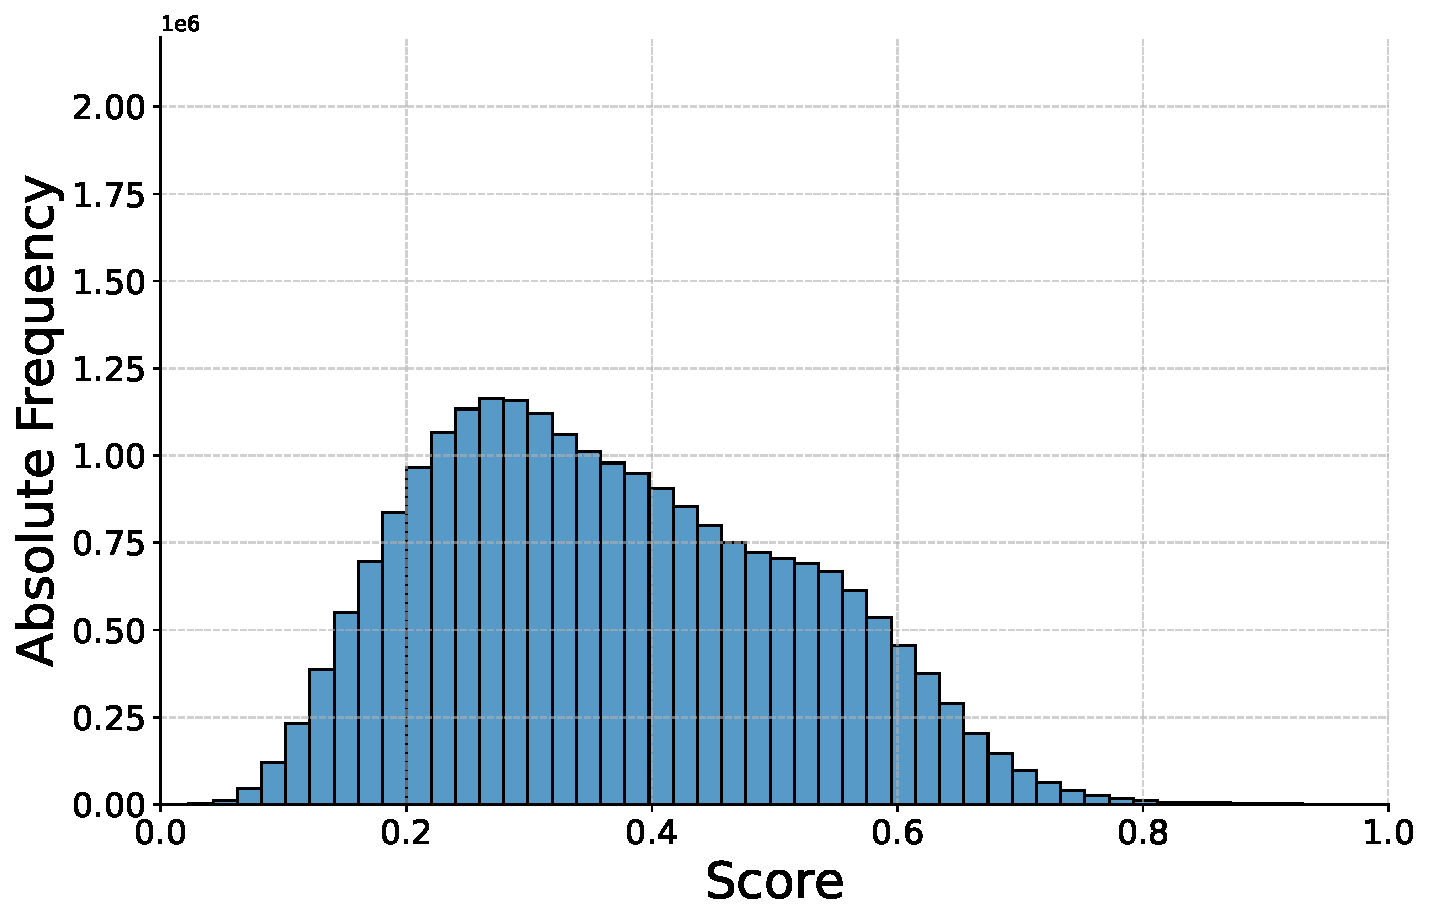
\includegraphics[width=\textwidth]{graphics/evaluation/pairwise_score_distribution_flan-t5-base.pdf}
        \label{fig:pairwise_flan-t5-base}
    \end{subfigure}
    \hfill
    \begin{subfigure}[b]{0.49\textwidth}
        \centering
        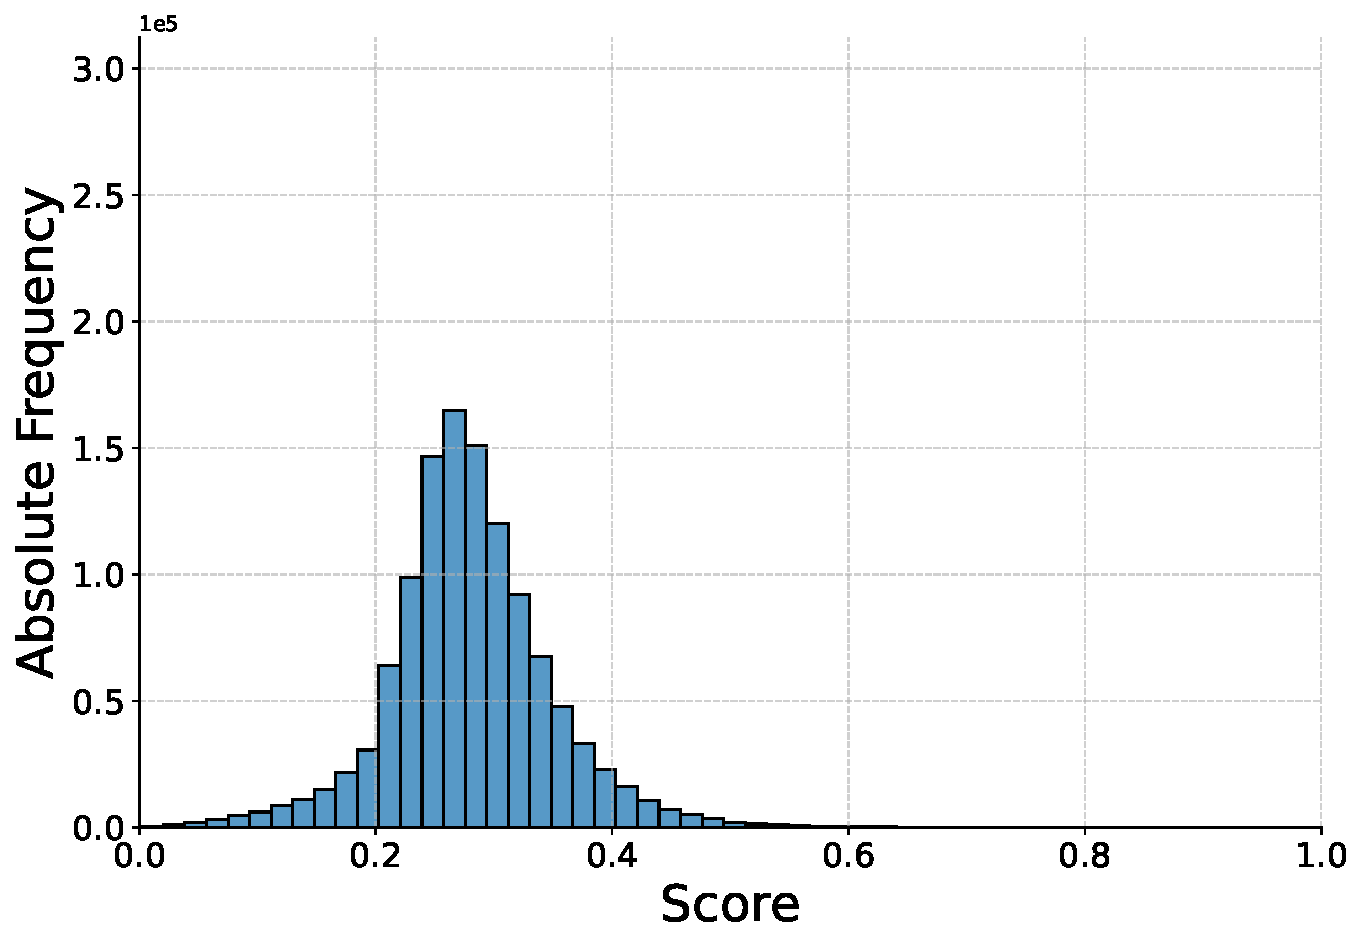
\includegraphics[width=\textwidth]{graphics/evaluation/pointwise_score_distribution_flan-t5-base.pdf}
        \label{fig:pointwise_flan-t5-base}
    \end{subfigure}

    \vspace{-0.5cm}
    \textbf{(a)} Relevance scores generated using \texttt{flan-t5-base}.
    \vspace{0.5cm}

    % Second row
    \begin{subfigure}[b]{0.49\textwidth}
        \centering
        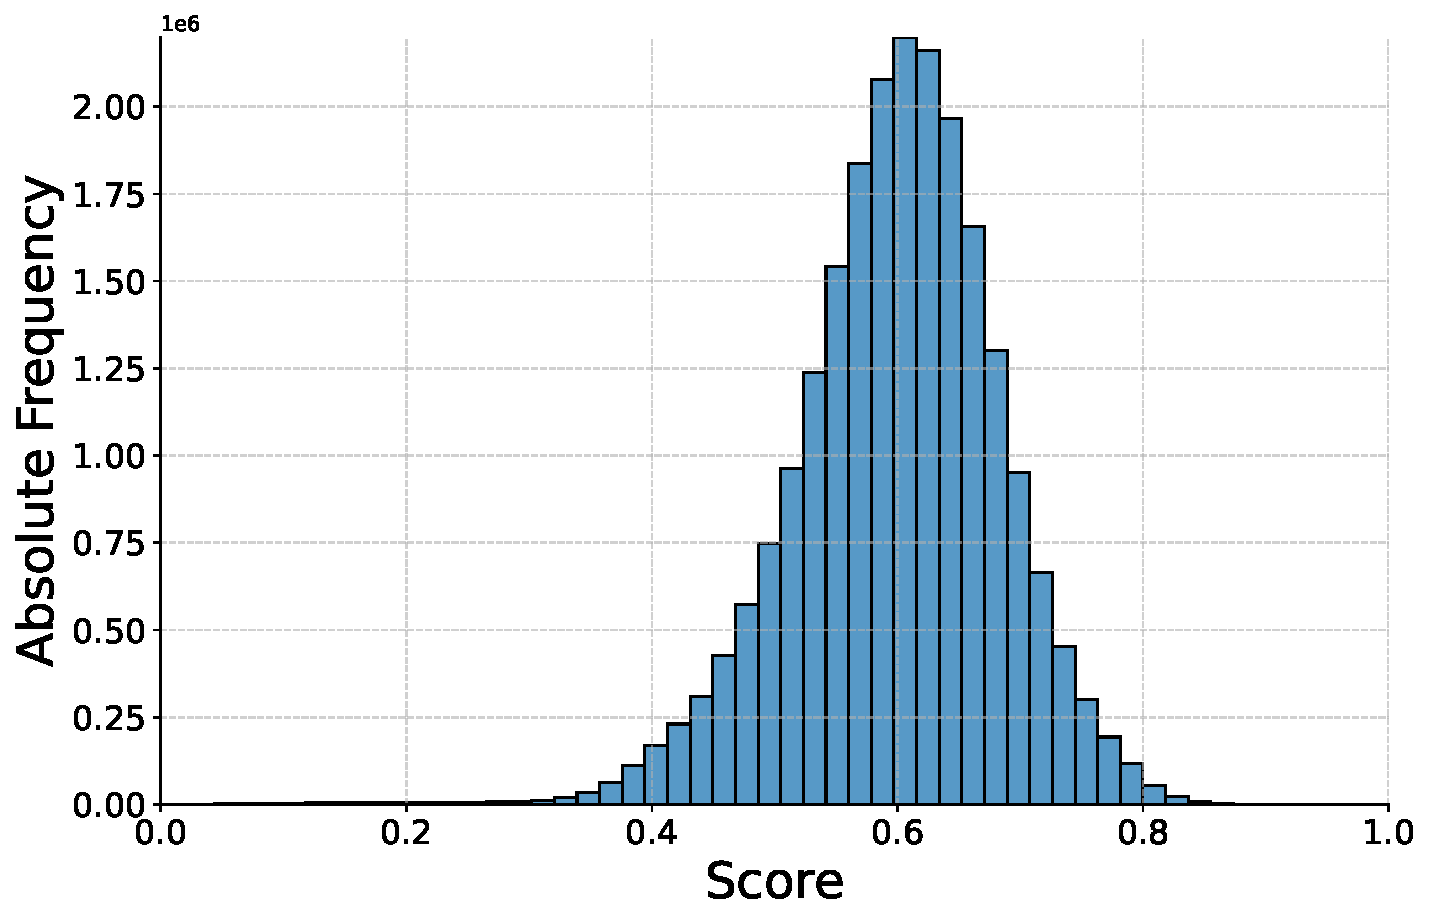
\includegraphics[width=\textwidth]{graphics/evaluation/pairwise_score_distribution_flan-t5-small.pdf}
        \label{fig:pairwise_flan-t5-small}
    \end{subfigure}
    \hfill
    \begin{subfigure}[b]{0.49\textwidth}
        \centering
        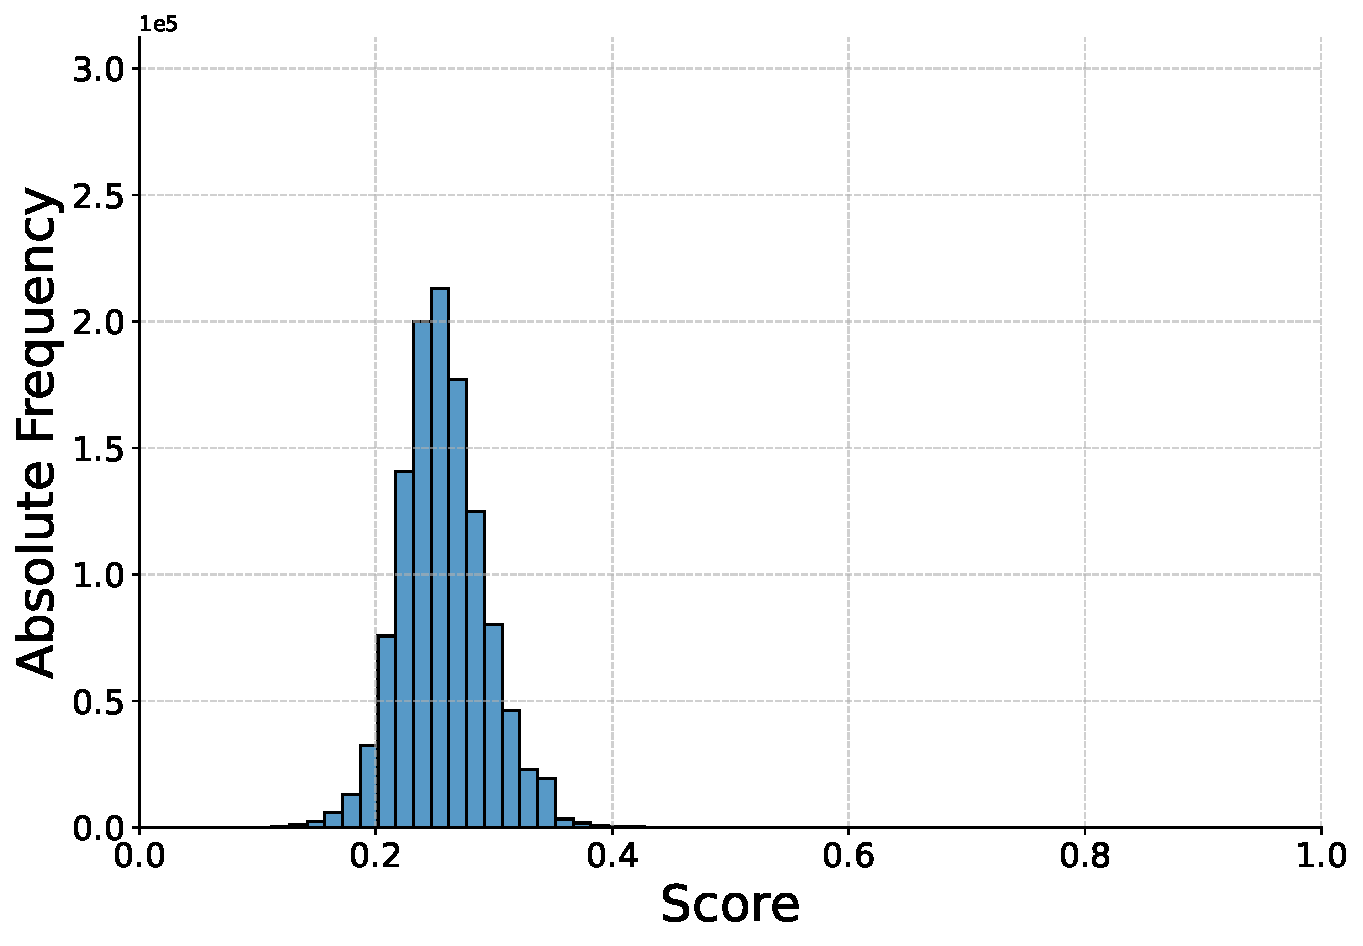
\includegraphics[width=\textwidth]{graphics/evaluation/pointwise_score_distribution_flan-t5-small.pdf}
        \label{fig:pointwise_flan-t5-small}
    \end{subfigure}

    \vspace{-0.5cm}
    \textbf{(b)} Relevance scores generated using \texttt{flan-t5-small}.
    \vspace{0.5cm}

    % Third row
    \begin{subfigure}[b]{0.49\textwidth}
        \centering
        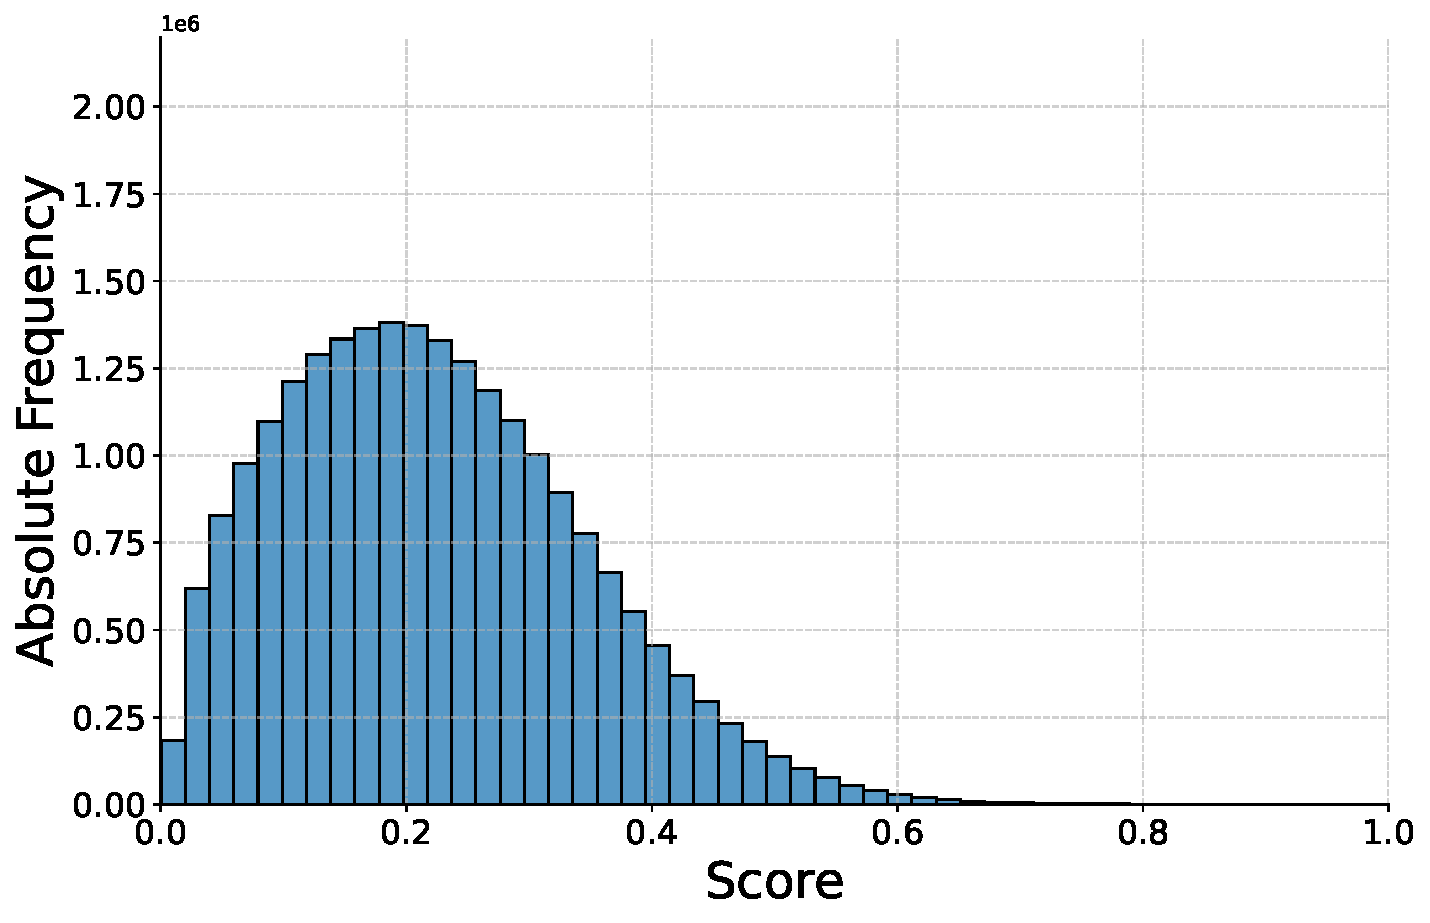
\includegraphics[width=\textwidth]{graphics/evaluation/pairwise_score_distribution_t5-small.pdf}
        \label{fig:pairwise_t5-small}
    \end{subfigure}
    \hfill
    \begin{subfigure}[b]{0.49\textwidth}
        \centering
        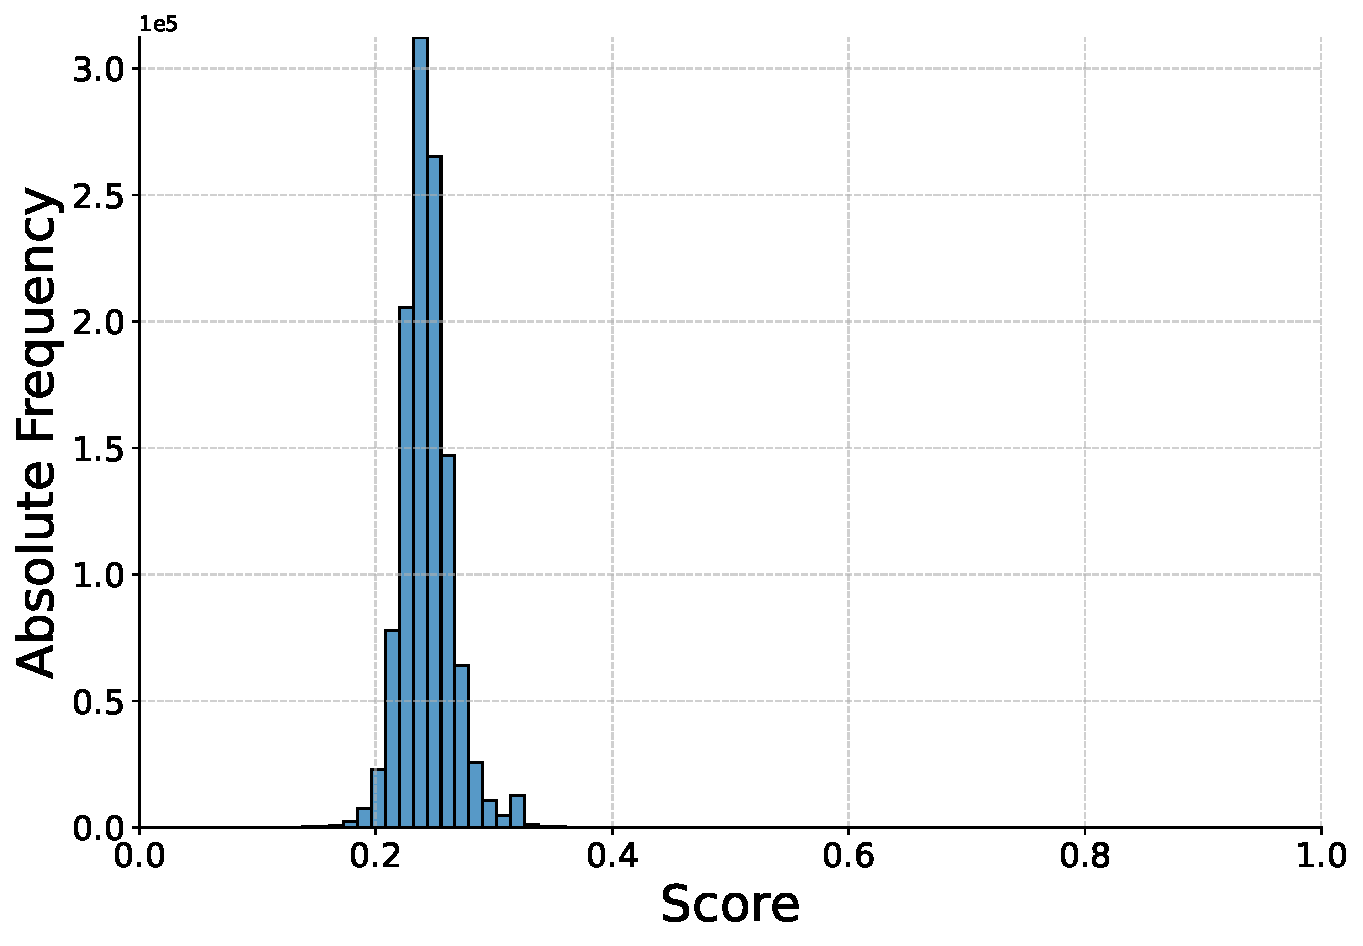
\includegraphics[width=\textwidth]{graphics/evaluation/pointwise_score_distribution_t5-small.pdf}
        \label{fig:pointwise_t5-small}
    \end{subfigure}

    \vspace{-0.5cm}
    \textbf{(c)} Relevance scores generated using \texttt{t5-small}.
    \vspace{0.5cm}

    \caption{Comparison of the distributions of the inferred relevance scores using the pairwise and pointwise approaches with different versions of the \texttt{T5} model.}
    \label{fig:score_distributions}
\end{figure}

% Transfer Pipeline to Source Corpus itself
\subsection{Transfer Pipeline on Source Corpora}\label{eval-pairwise-preferences-source}

% Transfer Pipeline to ClueWeb22/b
\subsection{Transfer Pipeline on \texttt{ClueWeb22/b}}\label{eval-pairwise-preferences-target}